\documentclass[14pt]{extarticle}

\usepackage[T1]{fontenc}
\usepackage[utf8]{inputenc}
\usepackage[russian]{babel}

% page margin
\usepackage[top=2cm, bottom=2cm, left=0.5cm, right=0.5cm]{geometry}

\usepackage{wrapfig}

% AMS packages
\usepackage{amsmath, array}
\usepackage{amssymb}
\usepackage{amsfonts}
\usepackage{amsthm}

\usepackage{graphicx}
\usepackage{rotating}

\usepackage{fancyhdr}
\pagestyle{fancy}
% modifying page layout using fancyhdr
\fancyhf{}
\renewcommand{\sectionmark}[1]{\markright{\thesection\ #1}}
\renewcommand{\subsectionmark}[1]{\markright{\thesubsection\ #1}}

\rhead{\fancyplain{}{\rightmark }}
\cfoot{\fancyplain{}{\thepage }}

\usepackage{titlesec}
\titleformat{\section}{\bfseries}{\thesection.}{1em}{}
\titleformat{\subsection}{\normalfont\itshape\bfseries}{\thesubsection.}{0.5em}{}

\newcommand{\pr}{\prime}
\newcommand{\lb}{\left(}
\newcommand{\rb}{\right)}

\newcommand{\intlonepi}{\int\limits_{0}^{\pi}}
\newcommand{\intltwopi}{\int\limits_{0}^{2\pi}}

\newcommand{\wvarphi}{\widetilde{\varphi}}
\newcommand{\wtheta}{\widetilde{\theta}}
\newcommand{\wpsi}{\widetilde{\psi}}

\usepackage{mathtools} % for dfrac!

\makeatletter
\def\env@dmatrix{\hskip -\arraycolsep
  \let\@ifnextchar\new@ifnextchar
  \extrarowheight=2ex
  \array{*\c@MaxMatrixCols{>{\displaystyle}c}}}

\newenvironment{dmatrix}
  {\env@dmatrix}
  {\endarray\hskip-\arraycolsep}

\newenvironment{bdmatrix}
  {\left[\env@dmatrix}
  {\endmatrix\right]}
% and other matrix environments are similar
\makeatother

\begin{document}

\section*{Группа вращений трехмерного пространства}

Рассмотрим все вращения трехмерного пространства вокруг фиксированной точки -- начала координат. Под произведением двух вращений $g_1$ и $g_2$ будем понимать вращение $g$, состоящее в последовательном применении сначала $g_2$ и затем $g_1$. Символически запишем это так: $g = g_1 g_2$. Нетрудно проверить, что совокупность $G$ всех вращений образует группу, т.е. что при таком определении умножения выполнены все групповые аксиомы. Единицей группы $e$, единичным вращением, является поворот на нулевой угол. \par

\section*{Описание группы вращений при помощи ортогональных матриц}

Пусть $x$ -- некоторый вектор, исходящий из начала координат, вращение $g$ переводит его в вектор $x^\pr$:
\begin{gather}
		x^\pr = g x \label{rotation_action}
\end{gather}

Рассмотрим ортогональную систему координат с центром в точке $O$, обозначим через $e_1$, $e_2$, $e_3$ единичные вектора, отложенные вдоль координатных осей. Вращение $g$ переводит эту тройку векторов в тройку других взаимно ортогональных векторов, которые будем обозначать $g_1$, $g_2$, $g_3$. Вектора $g_k$, $k =1, 2, 3$ задаются проекциями на оси $e_i$, $i = 1,2,3$; обозначим через $g_{ik} = ( g_k, e_i )$ проекцию вектора $g_k$ на $i$-ую ось. Объединим проекции в матрицу
\begin{gather}
	\begin{vmatrix}
		g_{11} & g_{12} & g_{13} \\
		g_{21} & g_{22} & g_{23} \\
		g_{31} & g_{32} & g_{33}
	\end{vmatrix}
	\label{rotation_matrix}
\end{gather}
Будем обозначать эту матрицу так же $g$ и называть ее матрицей вращения $g$. Выпишем соотношение \eqref{rotation_action} покоординатно
\begin{gather}
	x_i^\pr = \sum_{k = 1}^{3} g_{ik} x_k, \label{rotation_action_coords}
\end{gathя векторов}
где $x_k$ -- координаты вектора $x$, а $x_i^\pr$ -- координаты вектора $x^\pr$. Найдем, каким условиям должны удовлетворять числа $g_{ik}$. Так как вращение не меняет длин и углов, то оно не меняет скалярного произведения векторов. Таким образом, если $x^\pr = g x$ и $y^\pr = g y$, то
\begin{gather}
	\sum_{i = 1}^{3} x_i^\pr y_i^\pr = \sum_{k = 1}^{3} x_k y_k \label{scalar_product}
\end{gather}

Подставим в левую часть равенства \eqref{scalar_product} вместо $x_i^\pr$ и $y_i^\pr$ их выражения по формуле \eqref{rotation_action_coords}:
\begin{gather}
	\sum_{i, k, l} g_{ik} \, g_{il} \, x_k y_l = \sum_{k} x_k y_k \label{scalar_product2}
\end{gather}

Сравнивая коэффициенты при произведениях $x_k y_l$ в левой и правой частях, получаем:
\begin{gather}
	\sum_{i = 1}^{3} g_{ik} \, g_{il} = \delta_{kl}, \label{scalar_product3}
\end{gather}
где $\delta_{kl}$ -- кронекеровская дельта, определенная следующими соотношениями: $\delta_{kl} = 1$, если $ k = l$, $\delta_{kl} = 0$, если $k \neq l$. Равенство \eqref{scalar_product3} может быть записано в матричной форме:
\begin{gather}
		g^\top g = e \label{scalar_product4}
\end{gather}
или
\begin{gather}
		g^\top = g^{-1}. \label{scalar_product5}
\end{gather}
Матрицы, удовлетворяющие равенствам \eqref{scalar_product4}, \eqref{scalar_product5}, называются ортогональными матрицами. Если взять детерминант обеих частей равенства \eqref{scalar_product4}, то получим $\det \lb g^\top \rb \det \lb g \rb = 1$, т.е. $\rvert \det \lb g \rb \rvert^2 = 1$, и  
\begin{gather}
	\det \lb g \rb = \pm 1. \label{unit_determinant}
\end{gather}

Итак, группа вращений $G$ может быть реализована (представлена) как группа ортогональных матриц третьего порядка с единичным детерминантом. 

\section{Введение параметров в группу вращений}

Так как каждое вращение есть вращение вокруг некоторой оси, то оно может быть полностью определено путем задания оси вращения и задания угла поворота вокруг нее. Так, вращение может быть задано вектором $\xi = (\xi_1, \xi_2, \xi_3)$, направленным вдоль оси вращения и равным по величине углу поворота. Направление вектора будем выбирать так, чтобы угол поворота не превосходил $\pi$. Координаты векторов, описывающих всевозможные вращения, будут удовлетворять условию $\xi_1^2 + \xi_2^2 + \xi_3^2 \leqslant \pi^2$, и, значит, заполнять шар радиуса $\pi$. Ясно, что различные внутренние точки шара описывают различные вращения, а две диаметрально противоположные точки на поверхности сферы -- одно и то же вращение на угол $\pi$ (поворот на угол $\pi$ в двух противоположных направлениях приводит к одному и тому же результату). \par
\textit{Такой способ описания вращений выявляет топологическую структуру группы вращений, а именно, эта группа топологически эквивалентна шару, у которого отождествлены диаметрально противоположные точки границы.} 

Представленные выше результаты показывают, что вращение $g$ может быть описано при помощи девяти параметров, а именно элементами $g_{ik}$ матрицы вращения $g$; однако эти параметры не являются независимыми, они связаны соотношениями \eqref{scalar_product3}. Примером описания вращения при помощи независимых параметров являются углы Эйлера. \par
Пусть вращение $g$ переводит координатные оси $Ox$, $Oy$, $Oz$ в оси $Ox^\pr$, $Oy^\pr$, $Oz^\pr$. Обозначим линию пересечения плоскостей $xOy$ и $x^\pr O y^\pr$ через $Ol$ (ее принято называть \textit{линией узлов}). Придадим ей направление таким образом, чтобы наблюдатель, смотря вдоль заданного направления, видел угол между осями $Oz$ и $Oz^\pr$ (меньше $\pi$), отложенным против часовой стрелки. Это условие задает направление линии узлов во всех ситуциях, за исключением тех, в которых угол между осями $Oz$, $Oz^\pr$ равен 0 или $\pi$. \par
Обозначим через $\varphi$ угол между осью $Ox$ и линией узлов $Ol$, через $\psi$ -- угол между $Ol$ и осью $Ox^\pr$ и через $\theta$ -- между $Oz$ и $Oz^\prime$. Пусть $g_\varphi$ и $g_\psi$ обозначают вращения вокруг оси $Oz$, $g_\theta$ -- вращение вокруг оси $Ox$. \par
Вращение $g$ может быть представлено композицией $g = \widetilde{g}_\psi \widetilde{g}_\theta g_\varphi$ трех поворотов $g_\varphi$, $\widetilde{g}_\theta$, $\widetilde{g}_\psi$ вокруг осей $Oz$, $Ol$, $Oz^\pr$, соответственно. В результате вращения $g_\varphi$ ось $Ox$ совпадет с линией узлов $Ol$; ось $Oz$ перейдет в ось $Oz^\pr$ в результате вращения $\widetilde{g}_\theta$; вращение $\widetilde{g}_\psi$ переведет линию узлов $Ol$ в $Ox^\pr$ (ось $Oy$ в результате вращений $g_\varphi$ и $\widetilde{g}_\psi$ перейдет в $Oy^\pr$). \par
Повороты $\widetilde{g}_\theta$ и $\widetilde{g}_\psi$ были сделаны вокруг вспомогательных осей $Ol$ и $Oz^\pr$; представим их в виде поворотов относительно первоначальных осей $Ox$ и $Oz$. Поворот $\widetilde{g}_\theta$ является преобразованием новой системы координатных осей, полученной из первоначальной, действием $g_\varphi$, следовательно $\widetilde{g}_\theta = g_\varphi g_\theta g_\varphi^{-1}$. Аналогично, $\widetilde{g}_\psi = (\widetilde{g}_\theta g_\varphi) g_\psi (\widetilde{g}_\theta g_\varphi)^{-1}$. Подставим в выражение для композиции поворотов $g$:
\begin{gather}
	g = \widetilde{g}_\psi \widetilde{g}_\theta g_\varphi = ( \widetilde{g}_\theta g_\varphi ) g_\psi ( \widetilde{g}_\theta g_\varphi)^{-1} \widetilde{g}_\theta g_\varphi = \widetilde{g}_\theta g_\varphi g_\theta = g_\varphi g_\theta g_\psi
\end{gather}
\textit{То есть, последовательность поворотов на углы $\varphi$, $\theta$, $\psi$ вокруг вспомогательных систем осей, получаемых в результате осуществления каждого следующего поворота, эквивалентна последовательности поворотов относительно исходных осей, сделанных в обратном порядке $\psi$, $\theta$, $\varphi$.} \par 
Три угла $\varphi, \theta, \psi$ являются независимыми и полностью определяют поворот $g$. Согласно определениям, они изменяются в пределах, $0 \leqslant \varphi < 2 \pi$, $0 \leqslant \psi < 2 \pi$, $0 \leqslant \theta \leqslant \pi$. Разные наборы эйлеровых углов $(\varphi, \theta, \psi)$, взятые из этих интервалов, определяют разные повороты, за исключением случаев $\theta = 0$ и $\theta = \pi$. В этих особых случаях плоскости $xOy$ и $x^\pr O y^\pr$ совпадают, и линия их пересечения, линия узлов $Ol$, оказывается неопределена. Варьируя ориентацию линии узлов в плоскости, заключаем, что в случае $\theta = 0$ пары углов $(\varphi, \psi)$ и $(\varphi + \alpha, \psi - \alpha)$ определяют один и тот же поворот для любого $\alpha$; аналогично, в случае $\theta = \pi$ пары углов $(\varphi, \psi)$ и $(\varphi + \alpha, \psi + \alpha)$ эквивалентны для любого $\alpha$.  	
Выразим элементы матрицы поворота $g$ через углы Эйлера. Вспользуемся полученным выражением для поворота $g$ через повороты $g_\varphi$, $g_\theta$ и $g_\psi$ относительно исходной системы координат.
\begin{gather}
	g_\varphi = 
	\begin{bmatrix}
		\cos \varphi & - \sin \varphi & 0 \\
		\sin \varphi & \cos \varphi & 0 \\
		0 & 0 & 1
	\end{bmatrix}, 
	\quad 
	g_\theta =
	\begin{bmatrix}
		1 & 0 & 0 \\
		0 & \cos \theta & - \sin \theta \\
		0 & \sin \theta & \cos \theta
	\end{bmatrix},
	\quad 
	g_\psi = 
	\begin{bmatrix}
		\cos \psi & - \sin \psi & 0 \\
		\sin \psi & \cos \psi & 0 \\
		0 & 0 & 1
	\end{bmatrix} \notag
\end{gather}
\begin{gather}
	g = g_\varphi g_\theta g_\psi = 
	\begin{bmatrix}
		\cos \varphi \cos \psi - \cos \theta \sin \varphi \sin \psi & - \cos \varphi \sin \psi - \cos \theta \sin \varphi \cos \psi & \sin \varphi \sin \theta \\
		\sin \varphi \cos \psi + \cos \theta \cos \varphi \sin \psi & - \sin \varphi \sin \psi + \cos \theta \cos \varphi \cos \psi & - \cos \varphi \sin \theta \\
		\sin \psi \sin \theta & \cos \psi \sin \theta & \cos \theta
	\end{bmatrix} \notag
\end{gather}

Заметим, что замена $\lb \varphi, \theta, \psi \rb \rightarrow \lb \pi - \varphi, \theta, \pi - \psi \rb$ переводит матрицу $g$ в $g^\top = g^{-1}$. То есть, если поворот $g$ задан углами $\lb \varphi, \theta, \psi \rb$, то обратный поворот задается углами $\lb \pi - \varphi, \theta, \pi - \psi \rb$.  

\section*{Связь группы вращений с группой унитарных матриц второго порядка}

Покажем, что вращения трехмерного пространства можно описывать комплексными матрицами второго порядка. Для этого рассмотрим стереографическую проекцию сферы на плоскость -- каждой точке P сферы относится точка $\zeta$ в плоскости, лежащая на луче NP, исходящем из северного полюса N. Вращение трехмерного пространства вокруг центра сферы переводит друг в друга точки сферы и порождает тем самым некоторое преобразование в плоскости. 

\begin{wrapfigure}{R}{0.3\textwidth}
\centering
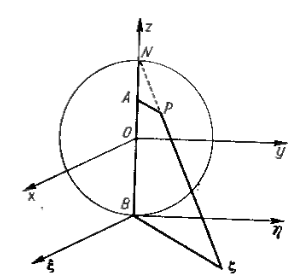
\includegraphics[width=0.25\textwidth]{pictures/stereographic.png}
\caption{\label{fig:stereographic}Стереографическая проекция}
\end{wrapfigure}

Рассмотрим сферу диаметра 1. Из подобия треугольников $\Delta$ANP и $\Delta$BN$\zeta$ получаем связь между координатами $x$, $y$, $z$ точки P сферы и координатами $\xi$, $\eta$ точки $\zeta$ плоскости:
\begin{gather}
	\xi = \frac{x}{\frac{1}{2} - z}, \qquad \eta = \frac{y}{\frac{1}{2} - z}. 
\end{gather}

Вводим комплексную переменную $\zeta = \xi + i \eta$:
\begin{gather}
	\zeta = \xi + i \eta = \frac{x + iy}{\frac{1}{2} - z} 
\end{gather}

Т.к. точка P принадлежит сфере единичного диаметра, то ее координаты $x$, $y$, $z$ удовлетворяют соотношению
\begin{gather}
	x^2 + y^2 + z^2 = \frac{1}{4}.
\end{gather}

Используем это соотношение при преобразовании $\zeta$:
\begin{gather}
	\zeta = \frac{x + iy}{\frac{1}{2} - z} = \frac{\lb x + iy \rb \lb x - iy \rb}{\lb \frac{1}{2} - z \rb \lb x - i y \rb} = \frac{x^2 + y^2}{\lb \frac{1}{2} - z \rb \lb x - iy \rb} = \frac{ \lb \frac{1}{2} - z \rb \lb \frac{1}{2} + z \rb}{ \lb \frac{1}{2} - z \rb \lb x - i y \rb} = \frac{ \frac{1}{2} + z }{ x - iy }.  
\end{gather}

Найдем преобразование плоскости, отвечающее вращению на угол $\varphi$ вокруг оси Oz. Имеем:
\begin{gather}
	\begin{aligned}
		x^\prime &= x \cos \varphi - y \sin \varphi \\
		y^\prime &= x \sin \varphi + y \cos \varphi \\
		z^\prime &= z
\end{aligned} \\
	\zeta^\prime = \frac{x^\prime + i y^\prime}{\frac{1}{2} - z} = \frac{ x (\cos \varphi + i \sin \varphi) + iy (\cos \varphi + i \sin \varphi)}{\frac{1}{2} - z} = \exp \lb i \varphi \rb \frac{x + iy}{\frac{1}{2} - z} = \exp \lb i \varphi \rb \zeta
\end{gather}

Т.е. вращению на угол $\varphi$ отвечает преобразование плоскости $\zeta^\prime = \exp \lb i \varphi \rb \zeta$. Рассмотрим вращение на угол $\theta$ вокруг оси Ox. Заметим, что при таком вращении выражение
\begin{gather}
	\omega = \frac{y + iz}{\frac{1}{2} - x}
\end{gather}
умножается на $\exp \lb i \theta \rb$, т.е.
\begin{gather}
	\omega^\prime = \exp \lb i \theta \rb \omega \label{omega_prime_with_omega}.
\end{gather}

Выразим $\omega$ через $\zeta$ (и соответственно $\omega^\prime$ через $\zeta^\prime$). Рассмотрим отношение:
\begin{gather}
		\frac{\omega + i}{\omega - i} = \frac{\displaystyle \frac{y + iz}{\frac{1}{2} - x} + i}{\displaystyle \frac{y + iz}{\frac{1}{2} - x} - i} = \frac{y + iz + i \lb \frac{1}{2} - x \rb}{y + iz - i \lb \frac{1}{2} - x \rb} = \frac{- \lb x + iy \rb + \lb z + \frac{1}{2} \rb}{\lb x - i y \rb + \lb z - \frac{1}{2} \rb }, \\
		x + iy = \zeta \lb \frac{1}{2} - z \rb, \quad x - iy = \lb z + \frac{1}{2} \rb \zeta^{-1} \\
		\frac{\omega + i}{\omega - i} = \frac{ \zeta \lb z - \frac{1}{2} \rb + \lb z + \frac{1}{2} \rb}{ \zeta^{-1} \lb z + \frac{1}{2} \rb + \lb z - \frac{1}{2} \rb} = \zeta \label{zeta_with_omega}
\end{gather}

Аналогично получаем
\begin{gather}
	\frac{\omega^\prime + i}{\omega^\prime - i} = \zeta^\prime. \label{zeta_prime_with_omega_prime}
\end{gather}

Выражаем $\omega$ через $\zeta$ в выражении \eqref{zeta_with_omega} и $\omega^\prime$ через $\zeta^\prime$ в выражении \eqref{zeta_prime_with_omega_prime}, подставляем выражения в соотношение \eqref{omega_prime_with_omega}, связывающее $\omega$ и $\omega^\prime$:   
\begin{gather}
	\omega = -i \frac{1 + \zeta}{1 - \zeta}, \qquad \omega^\prime = - i \frac{1 + \zeta^\prime}{1 - \zeta^\prime} \\
	\frac{\zeta^\prime + 1}{\zeta^\prime - 1} = \exp \lb i \theta \rb \frac{\zeta + 1}{\zeta - 1} 
\end{gather}

Решая это уравнение относительно $\zeta^\prime$, мы получаем преобразование, отвечающее вращения на угол $\theta$ вокруг оси Ox:
\begin{gather}
	\zeta^\prime = \frac{ \zeta \lb \exp \lb i \theta \rb + 1 \rb + \lb \exp \lb i \theta \rb - 1 \rb }{ \zeta \lb \exp \lb i \theta \rb - 1 \rb + \lb \exp \lb i \theta \rb + 1 \rb} \\ 
	\frac{ \exp \lb i \theta \rb + 1 }{ \exp \lb i \theta \rb - 1 } = \frac{ \exp \lb 2 i \theta \rb - 1 }{ \exp \lb 2 i \theta \rb - 2 \exp \lb i \theta \rb + 1 } = \frac{\exp \lb i \theta \rb - \exp \lb - i \theta \rb }{ \exp \lb i \theta \rb + \exp \lb -i \theta \rb - 2 } = -i \frac{\sin \theta}{1 - \cos \theta}  = - i \ctg \frac{\theta}{2} \notag \\
	\ctg \frac{\theta}{2} = \frac{\displaystyle \cos \frac{\theta}{2}}{\displaystyle \sin \frac{\theta}{2}} = \frac{\displaystyle 2 \sin \frac{\theta}{2} \cos \frac{\theta}{2}}{\displaystyle 2 \sin^2 \frac{\theta}{2}} = \frac{\sin \theta}{1 - \cos \theta} \notag
\end{gather}

\begin{gather}
		\zeta^\prime = \frac{\zeta \lb \exp \lb i \theta \rb + 1 \rb + \lb \exp \lb i \theta \rb - 1 \rb}{\zeta \lb \exp \lb i \theta \rb - 1 \rb + \lb \exp \lb i \theta \rb + 1 \rb} = \frac{\displaystyle \zeta \frac{\exp \lb i \theta \rb + 1}{\exp \lb i \theta \rb - 1} + 1}{\displaystyle \zeta + \frac{\exp \lb i \theta \rb + 1}{\exp \lb i \theta \rb - 1}} = \frac{\displaystyle -i \zeta \ctg \frac{\theta}{2} + 1}{\displaystyle \zeta - i \ctg \frac{\theta}{2}} \\ 
	\zeta^\prime = \frac{\displaystyle \zeta \cos \frac{\theta}{2} + i \sin \frac{\theta}{2}}{\displaystyle i \zeta \sin \frac{\theta}{2} + \cos \frac{\theta}{2}}
\end{gather}

Таким образом, мы видим, что вращениям вокруг осей Ox и Oz отвечают дробно-линейные преобразования в плоскости $\zeta$. Ясно, кроме того, что произведению вращений отвечает произведение преобразований в плоскости. Так как всякое вращение можно получить как произведение вращей вокруг осей Oz и Ox, то всякому вращению отвечает отвечает дробно-линейное преобразование общего вида
\begin{gather}
	\zeta^\prime = \frac{a \zeta + \beta}{\gamma \zeta + \delta}. \label{fractionlinear}
\end{gather}

Дробно-линейное преобразование \eqref{fractionlinear} однозначно определяется комплексной матрицей второго порядка
\begin{gather}
	\begin{bmatrix}
		\alpha & \beta \\
		\gamma & \delta
	\end{bmatrix}. \label{fractionlinearmatrix}
\end{gather}

Так как $\zeta^\prime$ из формулы \eqref{fractionlinear} не меняется при умножении числителя и знаменателя правой части на одно и то же число, то умножив $\alpha$, $\beta$, $\gamma$, $\delta$ на $\displaystyle \pm \frac{1}{\sqrt{\alpha \delta - \beta \gamma}}$, мы можем считать определитель матрицы \eqref{fractionlinearmatrix} равным 1. Таким образом, каждому вращению отвечает определенная с точностью до знака матрица вида \eqref{fractionlinearmatrix}, для которой $\alpha \delta - \beta \gamma = 1$. Выпишем матрицы, отвечающие вращениям $g_\varphi$ и $g_\theta$ вокруг осей Oz и Ox. Вращению $g_\theta$ отвечает матрица
\begin{gather}
	g_\theta \sim 
	\begin{bdmatrix}
		\cos \frac{\theta}{2} & i \sin \frac{\theta}{2} \\
		i \sin \frac{\theta}{2} & \cos \frac{\theta}{2}
	\end{bdmatrix} . \label{g_theta_matrix}
\end{gather}

Вращению $g_\varphi$ отвечает преобразование $\zeta^\prime = \exp \lb i \varphi \rb \zeta$. Записав его в виде $\displaystyle \zeta^\prime = \frac{\displaystyle \exp \lb \frac{i \varphi}{2} \rb \zeta}{\displaystyle \exp \lb -\frac{i \varphi}{2} \rb}$, мы получим матрицу преобразования
\begin{gather}
	g_\varphi \sim 
	\begin{bdmatrix}
		\exp \lb \frac{i \varphi}{2} \rb & 0 \\
		0 & \exp \lb - \frac{i \varphi}{2} \rb
	\end{bdmatrix} \label{g_varphi_matrix}
\end{gather}

с определителем, равным единице. \par
Вращение $g$ c эйлеровыми углами $\varphi$, $\theta$, $\psi$ может быть записано как произведение вращений $g = g_\varphi g_\theta g_\psi$. Пребразованию $g$ отвечает матрица
\begin{gather}
	g \sim
	\begin{bdmatrix}
		\exp \lb \frac{i \varphi}{2} \rb & 0 \\
		0 & \exp \lb - \frac{i \varphi}{2} \rb
	\end{bdmatrix}
	\begin{bdmatrix}
		\cos \frac{\theta}{2} & i \sin \frac{\theta}{2} \\
		i \sin \frac{\theta}{2} & \cos \frac{\theta}{2}
	\end{bdmatrix}
	\begin{bdmatrix}
		\exp \lb \frac{i \psi}{2} \rb & 0 \\
		0 & \exp \lb -i \frac{i \psi}{2} \rb
	\end{bdmatrix} = \notag \\
	= \begin{bdmatrix}
		\cos \frac{\theta}{2} \exp \lb \frac{i}{2} \lb \varphi + \psi \rb \rb & i \sin \frac{\theta}{2} \exp \lb - \frac{i}{2} \lb \psi - \varphi \rb \rb \\
		i \sin \frac{\theta}{2} \exp \lb \frac{i}{2} \lb \psi - \varphi \rb \rb & \cos \frac{\theta}{2} \exp \lb - \frac{i}{2} \lb \varphi + \psi \rb \rb
	\end{bdmatrix} \label{g_matrix}
\end{gather}

Матрицы \eqref{g_theta_matrix} и \eqref{g_varphi_matrix} являются унитарными матрицами с детерминантом 1. Поэтому и их произведение -- матрица \eqref{g_matrix}, отвечающая произвольному вращению, также униатрана и имеет детерминант, равный 1. \par
Покажем теперь, что, обратно, всякой унитарной матрице с единичным детерминантом отвечает некоторое вращение. Условия унитарности матрицы с элементами $\alpha$, $\beta$, $\gamma$, $\delta$ дают следующие соотношения  
\begin{gather}
	\begin{aligned}
		\alpha \alpha^{*} &+ \beta \beta^{*} = 1, \\
		\alpha \gamma^{*} &+ \beta \delta^{*} = 0, \\
		\gamma \alpha^{*} &+ \delta \beta^{*} = 0, \\
		\gamma \gamma^{*} &+ \delta \delta^{*} = 1.
	\end{aligned}
\end{gather}
Используем также условие единичности детерминанта:
\begin{gather}
	\alpha \delta - \beta \gamma = 1 \quad \implies \quad \alpha \alpha^{*} \delta - \alpha^{*} \beta \gamma = \alpha^{*} \notag \\
	\lb 1 - \beta \beta^{*} \rb \delta - \alpha^{*} \beta \gamma = \alpha^{*} \notag \\
	\lb 1 - \beta \beta^{*} \rb \delta + \beta \beta^{*} \delta = \alpha^{*} \quad \implies \alpha^{*} = \delta \notag \\
	\alpha \delta - \beta \gamma = 1 \quad \implies \quad \alpha \beta^{*} \delta - \beta \beta^{*} \gamma = \beta^{*} \notag \\
	\alpha \beta^{*} \delta - \lb 1 - \alpha \alpha^{*} \rb \gamma = \beta^{*} \notag \\
	- \alpha \alpha^{*} \gamma - \lb 1 - \alpha \alpha^{*} \rb \gamma = \beta^{*} \quad \implies \quad \gamma = - \beta^{*} \notag
\end{gather}

Поэтому произвольная матрица рассматриваемого типа может быть представлена в виде
\begin{gather}
	\begin{bmatrix}
		\alpha & \beta \\
		- \beta^{*} & \alpha^{*}
	\end{bmatrix}, \label{general_unit_rotation_matrix}
\end{gather}
где 
\begin{gather}
	\lvert \alpha \rvert^2 + \lvert \beta \rvert^2 = 1. \label{general_unit_rotation_matrix_condition}
\end{gather}

Ясно что матрицу \eqref{general_unit_rotation_matrix} при условии \eqref{general_unit_rotation_matrix_condition} можно представить в виде \eqref{g_matrix}, если положить (т.к. $0 \leqslant \theta \leqslant \pi$) 
\begin{gather}
	\cos \frac{\theta}{2} = \lvert \alpha \rvert, \quad \sin \frac{\theta}{2} = \lvert \beta \rvert, 
\end{gather}

а углы $\varphi$ и $\psi$ определить из уравнений
\begin{gather}
	\begin{aligned}
		\frac{1}{2} \lb \varphi + \psi \rb &= \arg \alpha, \\
		- \frac{1}{2} \lb \psi - \varphi \rb + \frac{\pi}{2} &= \arg \beta.
	\end{aligned}
\end{gather}

Таким образом, каждое вращение можно задавать двумя комплексными числами, удовлетворяющими условию \eqref{general_unit_rotation_matrix_condition}, или, что то же, четырьмя вещественными числами, сумма квадратов которых равна 1. \par
Итак, показано, что всякй унитарной матрице второго порядка с детерминантом 1 отвечает вращение в трехмерном пространстве. Обратно, всякому вращению отвечают \textit{две} такие матрицы, отличающиеся знаком. \par
Установленное ранее соответствие между вращениями и дробно-линейными преобразованиями однозначно. С другой стороны, мы видели, что каждое дробно-линейное преобразование может быть записано с помощью двух матриц с детерминантом, равным 1. Таким образом, каждому вращению отвечают \textit{две} матрицы вида \eqref{general_unit_rotation_matrix}. Естественного способа избавиться от двузначности этого соотвествия нет. Рассмотрим, например, вращение на угол $\varphi$ вокруг оси Oz. Ему отвечает матрица 
\begin{gather}
	\begin{bdmatrix}
		\exp \lb \frac{i \varphi}{2} \rb & 0 \\
		0 & \exp \lb - \frac{i \varphi}{2} \rb 
	\end{bdmatrix}.
\end{gather}

В частности, единичному вращению $\varphi = 2 k \pi$ отвечают две матрицы 
\begin{gather}
	\begin{bmatrix}
		\pm 1 & 0 \\
		0 & \pm 1
	\end{bmatrix}. \label{unit_rotation_matrices}
\end{gather}

Если бы мы сопоставили этому вращению лишь матрицу 
\begin{gather}
	\begin{bmatrix}
		1 & 0 \\
		0 & 1
	\end{bmatrix},
\end{gather}

то, изменяя угол $\varphi$ непрерывно от $0$ до $2 \pi$, мы пришли бы при $\varphi = 2 \pi$ к матрице
\begin{gather}
	\begin{bmatrix}
		-1 & 0 \\
		0 & -1 
	\end{bmatrix} .
\end{gather}

Таким образом, для сохранения непрерывности мы должны считать, что единичному вращению отвечают обе матрицы \eqref{unit_rotation_matrices}. 

\section*{Инвариантный интеграл на группе вращений}

Будем говорить, что задана функция $\omega = f(g)$ на группе $G$, если каждому вращению $g \in G$ отвечает некоторое число $\omega$. Если задавать вращение $g$ эйлеровыми углами $\varphi$, $\theta$, $\psi$, то $f(g)$ станет просто функцией от $\varphi$, $\theta$, $\psi$:
\begin{gather}
	f(g) = f(\varphi, \theta, \psi), \notag
\end{gather}
причем
\begin{gather}
	f(\varphi + 2 \pi, \theta, \psi) = f(\varphi, \theta, \psi + 2 \pi) = f( \varphi, \theta, \psi). \notag
\end{gather}

Инвариантным интегралом функции $f(g)$ на группе $G$ называют интеграл
\begin{gather}
		\int\limits_{0}^{2\pi} \int\limits_{0}^{\pi} \int\limits_{0}^{2\pi} f(g) \omega(g) \, d \varphi \, d\theta \, d\psi = \int\limits_{0}^{2\pi} \int\limits_{0}^{\pi} \int\limits_{0}^{2\pi} f(\varphi, \theta, \psi) \omega( \varphi, \theta, \psi) \, d\varphi \, d\theta \, d\psi, 
\end{gather}
в котором множитель $\omega(g)$ выбран так, чтобы для любой функции $f(g) = f(\varphi, \theta, \psi)$, непрерывной относительно $\varphi, \theta, \psi$, выполнялось условие
\begin{gather}
	\intltwopi \intlonepi \intltwopi f(g g_0) \omega (g) \, d\varphi \, d\theta \, d\psi = \intltwopi \intlonepi \intltwopi f(g) \omega(g) \, d\varphi \, d\theta \, d\psi \label{invariant_integration_condition}  
\end{gather}

Непосредственным вычислением можно показать, что множитель $\omega(g)$  этим условием определяется однозначно с точностью до числового множителя (интересно, как?). Этот результат вытекает также без всяких вычислений из общий теории интегрирования на топологической группе \cite{weil}. Покажем, что функция
\begin{gather}
	\omega(g) = \sin \theta \quad \textup{при} \quad g = g_\varphi g_\theta g_\psi  
\end{gather}
удовлетворяет условию \eqref{invariant_integration_condition}, так что выражение 
\begin{gather}
	\intltwopi \intlonepi \intltwopi f(g) \sin \theta \, d\varphi \, d\theta \, d\psi \label{invariant_integration_weight}
\end{gather}
есть инвариантный интеграл на группе $G$. Положим $\widetilde{g} = g g_0$ и обозначим через $\widetilde{\varphi}$, $\widetilde{\theta}$, $\widetilde{\psi}$ эйлеровы углы вращения $\widetilde{g}$; очевидно, $\widetilde{\varphi}$, $\widetilde{\theta}$, $\widetilde{\psi}$ являются функциями эйлеровых углов $\varphi$, $\theta$, $\psi$ вращения $g$, и условие \eqref{invariant_integration_condition} для интеграла \eqref{invariant_integration_weight} означает, что должно быть 
\begin{gather}
	\intltwopi \intlonepi \intltwopi f( \widetilde{\varphi}, \widetilde{\theta}, \widetilde{\psi}) \sin \theta \, d\varphi \, d\theta \, d\psi = \intltwopi \intlonepi \intltwopi f(\varphi, \theta, \psi) \sin \theta \, d \varphi \, d\theta \, d\psi. 
\end{gather}

\begin{wrapfigure}{R}{0.3\textwidth}
\centering
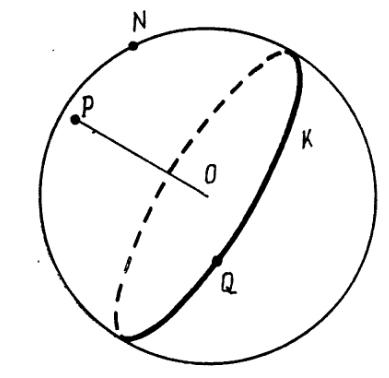
\includegraphics[width=0.25\textwidth]{pictures/change_of_variables.png}
\caption{\label{fig:change_of_variables}}
\end{wrapfigure}

Переходя в интеграле слева от переменных интегрирования $\varphi$, $\theta$, $\psi$ к переменным $\widetilde{\varphi}$, $\widetilde{\theta}$, $\widetilde{\psi}$, видим, что он будет равен интегралу в правой части, если при этом преобразовании переменных $\sin \theta \, d\varphi \, d\theta \, d\psi$ преобразуется в $\sin \widetilde{\theta} \, d\widetilde{\varphi} \, d\widetilde{\theta} \, d\widetilde{\psi}$, т.е. если
\begin{gather}
	\sin \wtheta \, d\wvarphi \, d\wtheta \, d\wpsi = \sin \theta \, d\varphi \, d\theta \, d\psi. \label{change_of_variables} 
\end{gather}

Обозначим через P точку на единичной сфере, в которую в результате вращения $g^{-1} = g^\top$ переходит северный полюс N$(0,0,1)$, а через Q -- точку, в которую в результате вращения $g^\top$ переходит точка $(1, 0, 0$). Вращение $g$ полностью определяется точками P, Q, причем точку P можно выбирать произвольным образом на сфере, а точку Q после этого -- произвольным образом на большом круге K, плоскость которого перпендикулярна к радиусу OP (так как образы векторов OP, OQ будут перпендикулярны). В результате применения матрицы $g^\top$ вектор $(0, 0, 1)$ переходит в вектор $(g_{31}, g_{32}, g_{33}) = (\sin \psi \sin \theta, \cos \psi \sin \theta, \cos \theta)$. Следовательно $\displaystyle \frac{\pi}{2} - \psi, \theta$ -- сферические координаты точки P; $dS = \sin \theta \, d \psi \, d \theta$ есть элемент площади поверхности сферы в точке P (в силу соотношения $\displaystyle dS = \Bigl\lvert \frac{\partial \mathbf{r}}{\partial \theta} \times \frac{\partial \mathbf{r}}{\partial \psi} \Bigr\rvert $). $d\varphi$ есть элемент дуги круга K, так как изменение $\varphi$ на $d\varphi$ (при фиксированных $\theta$, $\psi$) не приведет к изменению положения точки P; ему отвечает вращение на $d\varphi$ вокруг OP, т.е. сдвиг точки Q на $d\varphi$.  

\begin{gather}
	Q =
	\begin{bmatrix}
		\cos \varphi \cos \psi - \cos \theta \sin \psi \sin \varphi \\
		-\cos \varphi \sin \psi - \cos \theta \sin \varphi \cos \psi \\
		\sin \varphi \sin \theta
	\end{bmatrix} \\ 
	dQ \biggr\rvert_{\substack{\psi = \text{const} \\ \theta = \text{const}}} =
	\begin{bmatrix}
		- \sin \varphi \cos \psi - \cos \theta \sin \psi \cos \varphi \\
		\sin \varphi \sin \psi - \cos \theta \cos \psi \cos \varphi \\
		\sin \theta \cos \varphi
	\end{bmatrix} d\varphi
\end{gather}
\begin{gather}
	\left[ dQ \biggr\rvert_{\substack{\psi = \text{const} \\ \theta = \text{const}}} \, \right]^2 = \lb d\varphi \rb^2  
	\quad \implies \quad
	dQ \biggr\rvert_{\substack{\psi = \text{const} \\ \theta = \text{const}}} = d\varphi
\end{gather}

Но точки $\widetilde{\text{P}}$ и $\widetilde{\text{Q}}$, отвечающие вращению $\widetilde{g} = g g_0$, получаются из точек P и Q вращением $g_0^\top$. При этом вращении и элемент $dS = \sin \theta \, d\theta \, d\psi$ площади поверхности сферы, и элемент $d\varphi$ дуги круга K остаются инвариантными; следовательно их произведение $\sin \theta \, d \varphi \, d \theta \, d\psi$ также остается инвариантным, чем и доказывается формула \eqref{change_of_variables}. \par

Очевидно, при любом положительном постоянном $c$ вес $\omega(g) = c \sin \theta$ также удовлетворяет условию \eqref{invariant_integration_condition}. Выберем $c$ так, чтобы выполнялось условие
\begin{gather}
	\intltwopi \intlonepi \intltwopi c \sin \theta \, d\varphi \, d\theta \, d \psi = 1, \label{invariant_integration_norm}
\end{gather}
т.е.
\begin{gather}
		c = \frac{1}{8 \pi^2}, \quad \omega(g) = \frac{1}{8 \pi^2} \sin \theta. 
\end{gather}

Выражение $\displaystyle \frac{1}{8 \pi^2} \sin \theta \, d\varphi \, d\theta \, d\psi$ называют элементом инвариантного объема на группе $G$ и обозначают через $dg$.  Условие инвараинтности \eqref{invariant_integration_condition} примет тогда вид
\begin{gather}
	\int f(g g_0) dg = \int f(g) dg. \label{invariant_integration_final_result} 
\end{gather}

Отметим, что, кроме того,
\begin{gather}
	\int f(g^{-1}) dg = \int f(g) dg \label{invariant_integration_inverse_rotation}
\end{gather}
и
\begin{gather}
	\int f(g_0 g) dg = \int f(g) dg.
\end{gather}

Действительно, переходу от $g$ к $g^{-1}$ отвечает переход от $\varphi, \theta, \psi$ к $\pi - \varphi, \theta, \pi - \psi$, в результате которого выражение $\sin \theta \, d\varphi \, d\theta \, d\psi$ не изменяется; отсюда следует формула \eqref{invariant_integration_inverse_rotation}.  


\nocite{naimark}
\nocite{gelfand}

\newpage
\bibliographystyle{plain}
\bibliography{biblio}

\end{document}

